\clearpage
\markboth{Problem 4}{Problem 4: Part 5}

\textbf{Problem Statement:} Consider the equation
$$f(x) = 0,$$
where
$$f(x) = x - \frac{1}{2}\left(\cos(x/2) - \left|x - \frac{1}{2}\right|\right).$$

Do the following.

\subsection*{Part 5}
\addcontentsline{toc}{subsection}{Problem 4.5}

Note the number of iterations needed to calculate the solution to within 10 decimal places using the Newton's method. Discuss the speed of convergence of the Newton's method and compare it with the convergence speed of the fixed point iterations.

\noindent\rule{\textwidth}{0.4pt}

\vspace{1em}

\textbf{Solution:}

The table below (see \Cref{tab:p04-5-newton-fpi}) shows the trajectory of $x_n$ and errors for Newton's method and FPI, starting from $x_0 = 0.48$.

\begin{table}[H]
    \centering
    \begin{tabular}{cccc}
        \toprule
        $n$ & $x_n$ & $e_n$ & $e_{n+1}/e_n^2$ \\
        \midrule
        $0$ & $0.4800000000$ & $7.748\times 10^{-3}$ & $1.086\times 10^{-1}$ \\
        $1$ & $0.4722581088$ & $6.517\times 10^{-6}$ & $8.519\times 10^{-1}$ \\
        $2$ & $0.4722515915$ & $3.619\times 10^{-11}$ & $-$ \\
        \bottomrule
    \end{tabular}
    \caption{Convergence of Newton's method for $f(x)$, showing rapid quadratic convergence.}
    \label{tab:p04-5-newton-fpi}
\end{table}

Newton's method converges to the root in just 3 iterations, while FPI requires 23. This demonstrates the dramatic efficiency advantage of Newton's method for this problem.

\vspace{2em}

% Insert convergence figure
\begin{figure}[H]
    \centering
    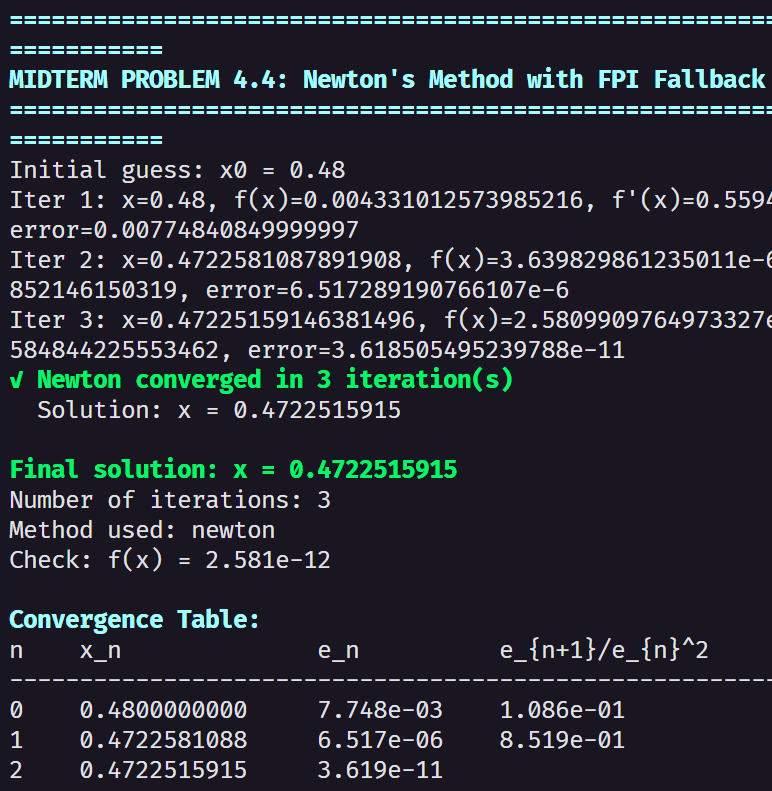
\includegraphics[width=0.55\textwidth]{figures/p04-4-newtons-method-convergence-terminal-output.png}
    \caption{Newton's method convergence output for $x_0=0.48$. The trajectory never reaches $x=0.50$.}
    \label{fig:p04-4-newton-convergence}
\end{figure}

As shown in \Cref{fig:p04-4-newton-convergence}, the sequence starting from $x_0=0.48$ converges rapidly and does not encounter $x=0.50$.

\vspace{2em}
\noindent\rule{\textwidth}{0.4pt}